

\newlength\myindent
\setlength\myindent{2em}
\newcommand\bindent{%
  \begingroup
  \setlength{\itemindent}{\myindent}
  \addtolength{\algorithmicindent}{\myindent}
}
\newcommand\eindent{\endgroup}



\appendix
\section{Supplementary Material: Figures}
The source code for the dynamic honeycomb maze is linked in a  \href{https://github.com/casualcoffeeaddict/Honeycomb-Maze}{\textit{github} repository},\\ at \href{https://github.com/casualcoffeeaddict/Honeycomb-Maze}{https://github.com/casualcoffeeaddict/Honeycomb-Maze}

This package was developed in \textit{Python} version 3.9.0 \cite{python3}, with integration from \textit{networkx} version 2.8 \cite{networkx}.

\subsection{Network of Integration}
\label{fig:integration_network}
\begin{figure}[H]
    \centering
    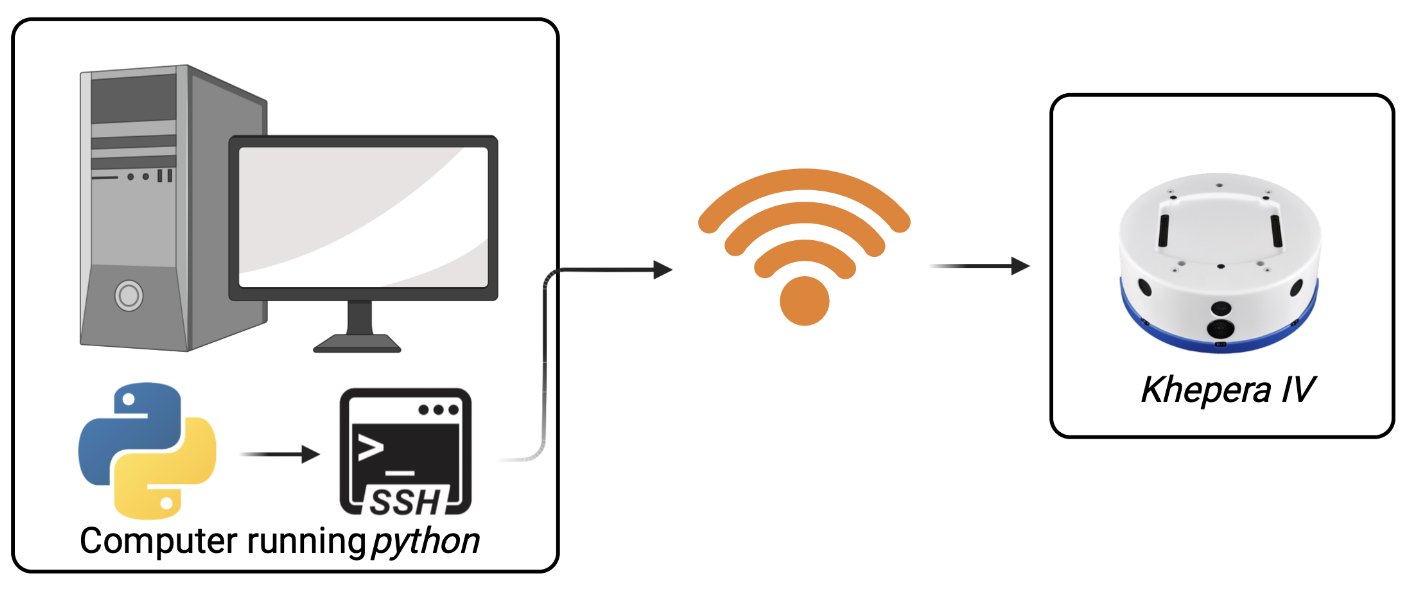
\includegraphics[scale = 0.6]{images/intergration_netwwork.png}
    \caption{This figure shows how the different components of the program integrate with each-other.}

\end{figure}

\subsection{Slice through cube}
\label{fig:hexagona_slice_through_cube}
\begin{figure}[H]
    \centering
    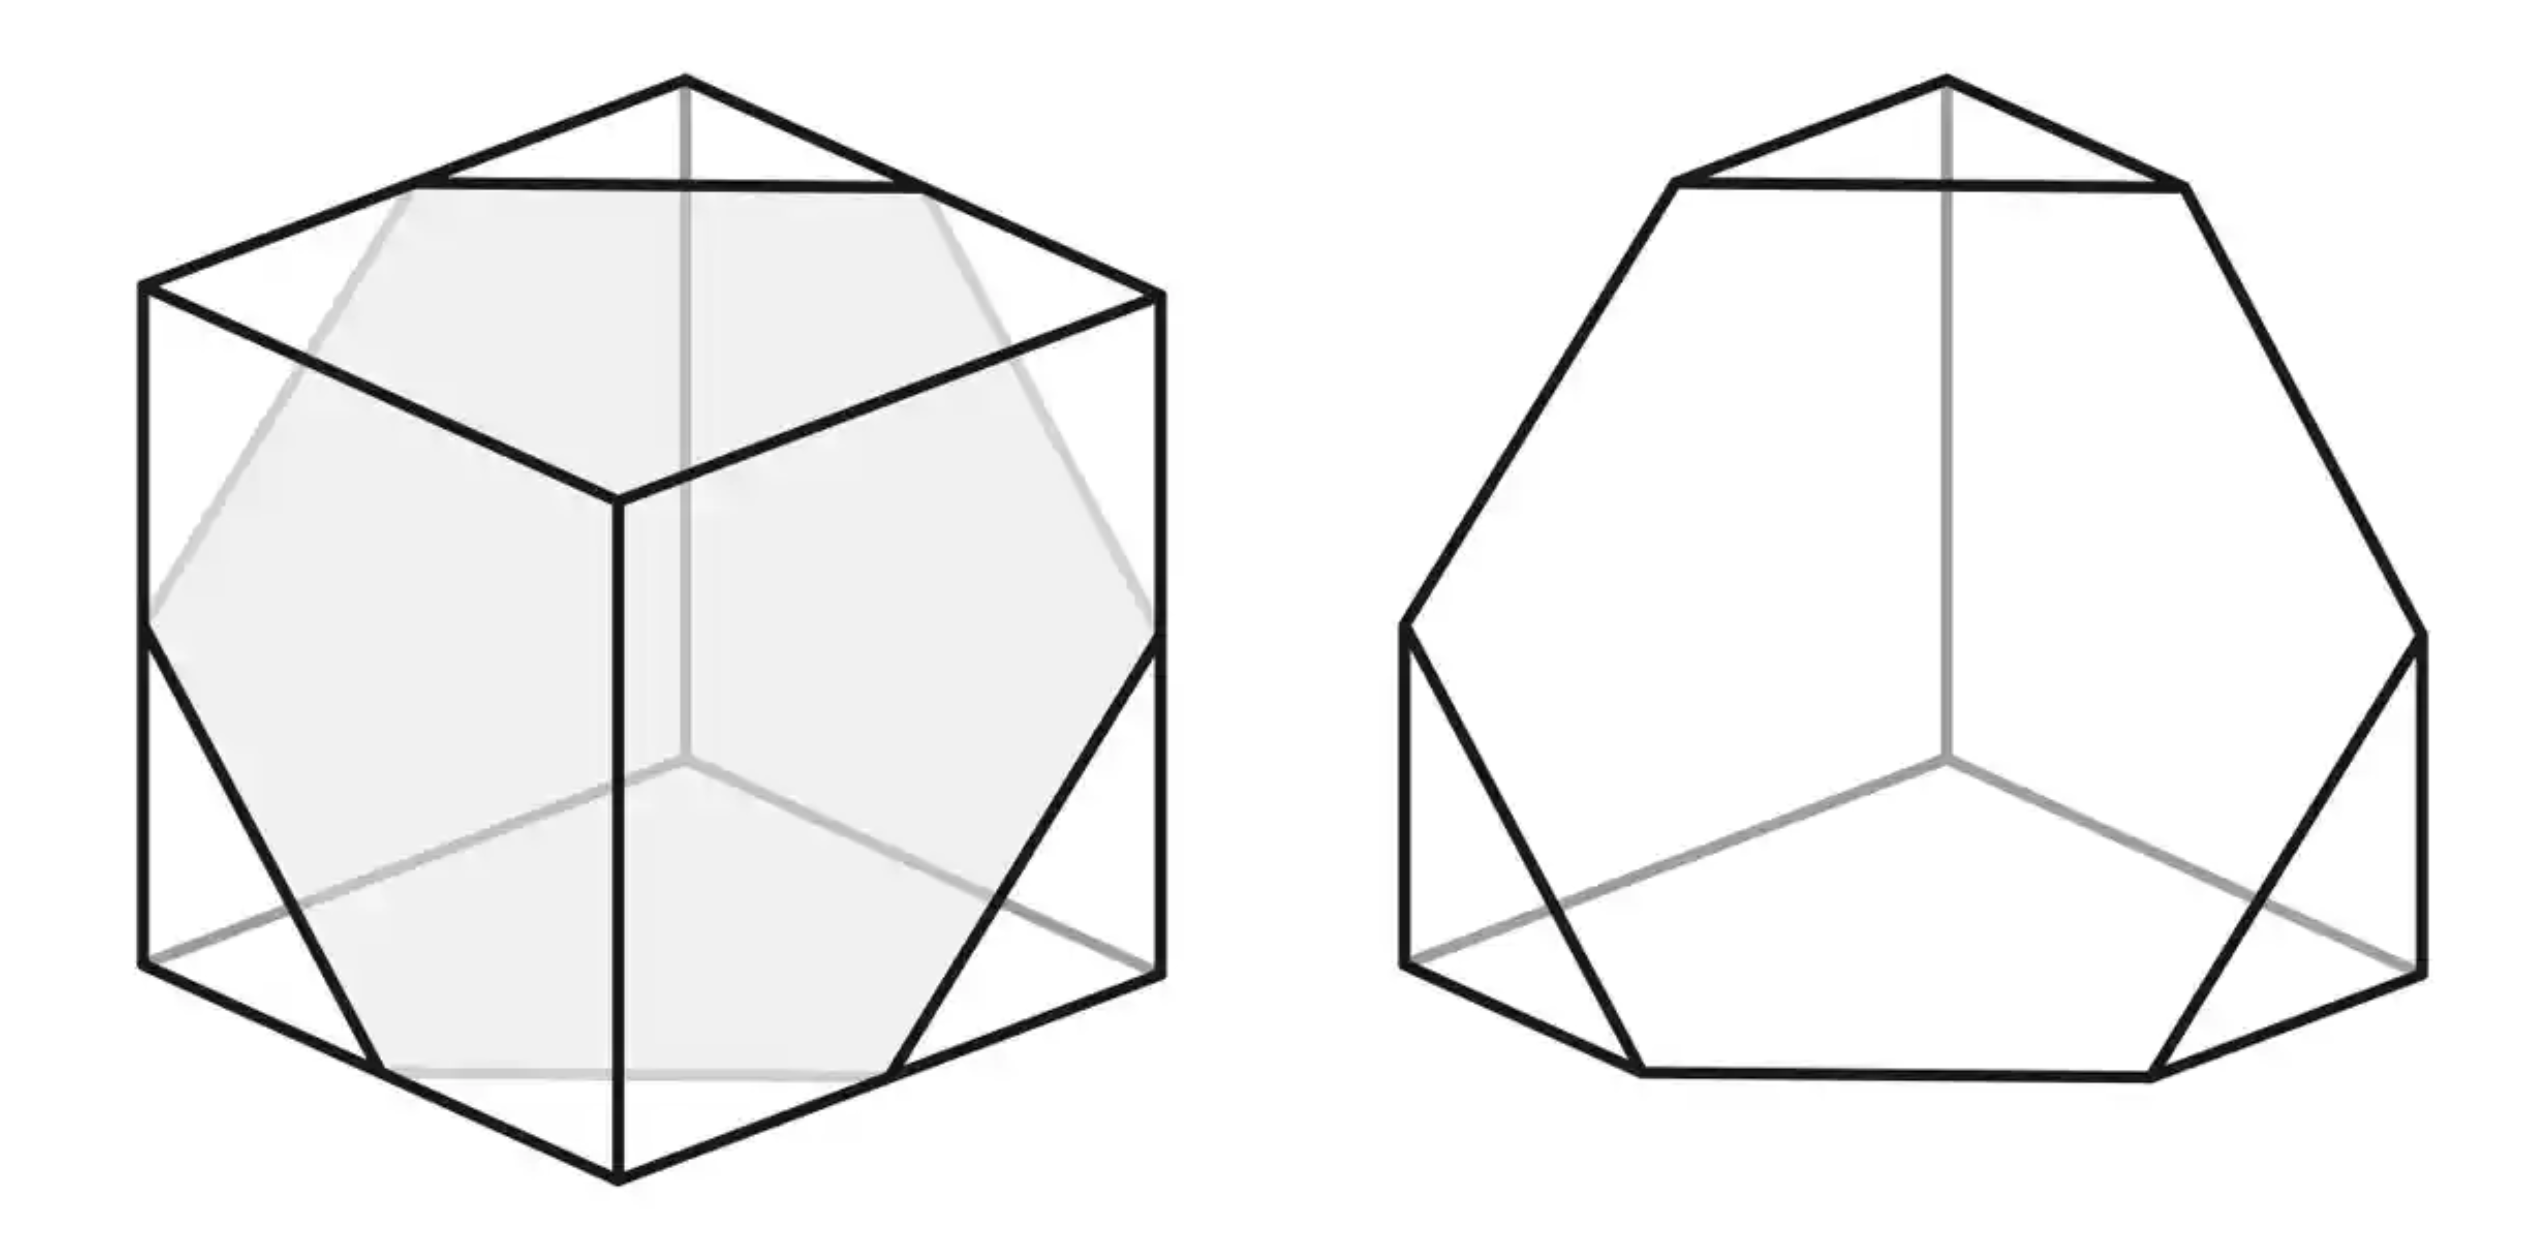
\includegraphics[scale = 0.3]{images/hexagonal_slice_through_cube.png}
    \caption{This is the slice  $x + y + z = 0$ through a cube. From this image it is clear that this plane through 3D space leaves a hexagon. This coordinate system used follows from this observation.}

\end{figure}

% \subsection{Truth Table for changing relative position}
% \label{table:relative_position_truth_table}

% \begin{tabular}{|c||c|c|c|}
%     % \centering
%     \hline
%     \multicolumn{4}{|c|}{Relative Position Truth Table} \\
%     \hline
%     Axis that is constant & x-axis & y-axis & z-axis \\
%     \hline
%     Relative Position    & 0 \&  3 & 1 \& 4 & 2 \& 5 \\
%     \hline
% \end{tabular}


\begin{figure}[H]
\label{table:change_states_of_robot}
\subsection{Truth Table for changing the states of the robots}
\begin{displaymath}
\begin{array}{|c| c||c|}
% |c c|c| means that there are three columns in the table and
% a vertical bar ’|’ will be printed on the left and right borders,
% and between the second and the third columns.
% The letter ’c’ means the value will be centered within the column,
% letter ’l’, left-aligned, and ’r’, right-aligned.
Previously AR & Currently AR & New State\\ % Use & to separate the columns
\hline % Put a horizontal line between the table header and the rest.
True & True & AR\\
True & False & NAR\\
False & True & AR\\
False & False & NNAR\\
\end{array}
\end{displaymath}

\caption{This Table shows how the states of the robot platforms will change based on their previous state and if they have been selected by the animal to become the new animal robot. AR = Animal Robot, NAR = Non Animal Robot and NNAR = Non-Non Animal Robot}
\end{figure}




\subsection{All platform positions the maze must deal with}
\label{fig:all_post_decision_states}
\begin{figure}[H]
    \centering
    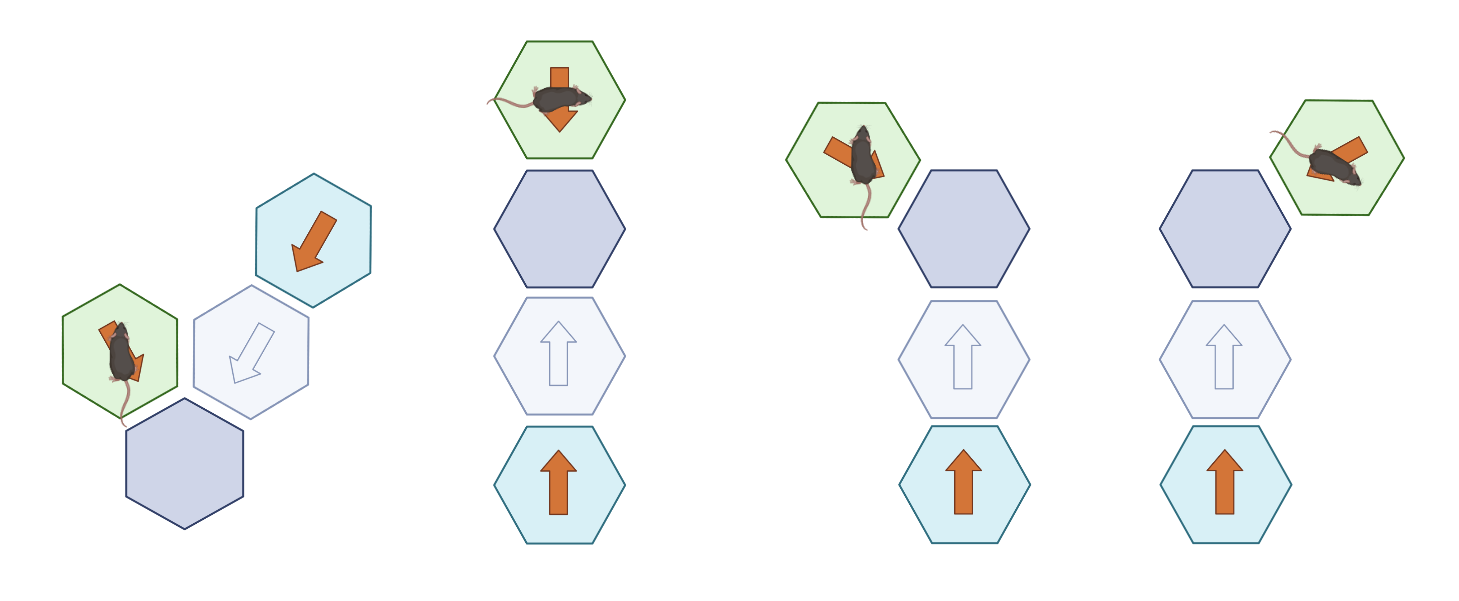
\includegraphics[scale = 0.32]{images/all_post_decision_states.png}
    \caption{This shows all the possible decision states that are possible after the animal has made a decision about which platform to move to, if states which are rotationally symmetric are removed. Since the two most left hand side figures are mirror images of each other, the same algorithm applies to both. This reduces the number of possibilities that need to be handled.}
\end{figure}


\subsection{Example path which the platforms will take through the hexagonal grid}
\label{fig:example_path}
\begin{figure}[H]
    \centering
    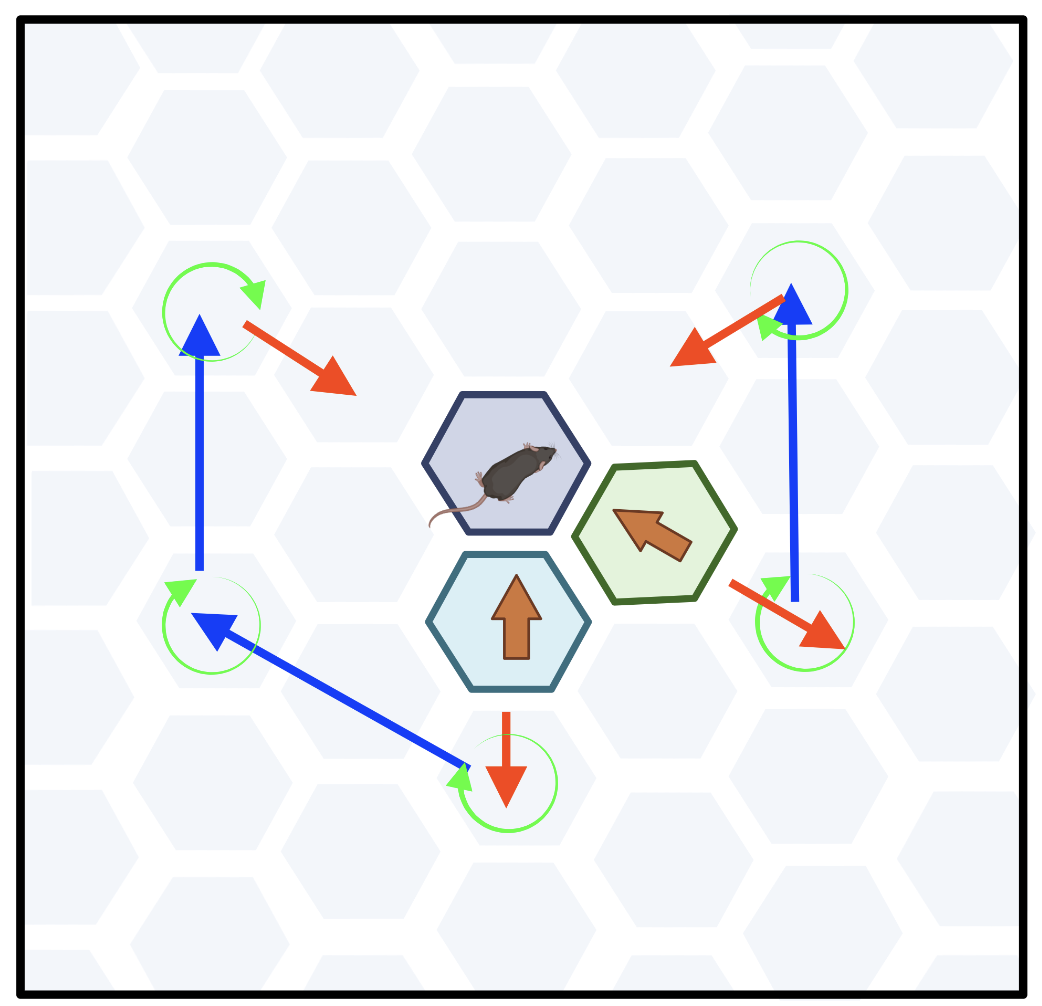
\includegraphics[scale=0.4]{images/overview_of_algorithm.png}
    \caption{This shows an example of the overall movement that would occur when moving the robot around}
    \label{fig:overview_of_algorithm}
\end{figure}



\subsection{Example of consecutive hexagonal platforms colliding}
\label{fig:collision}
\begin{figure}[H]
    \centering
    % 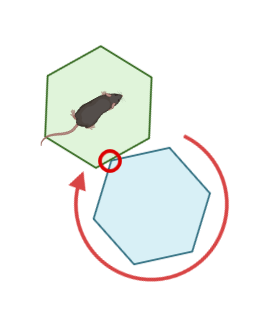
\includegraphics[scale = 0.5]{images/consec_hex_collision .png}
    % 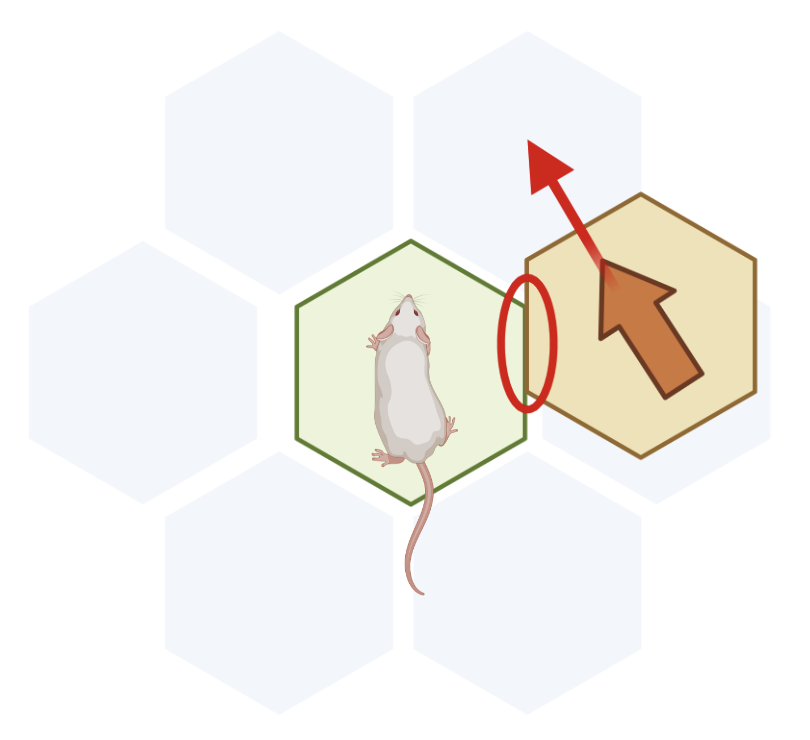
\includegraphics[scale = 0.25]{images/direct_inner_movement.png}
    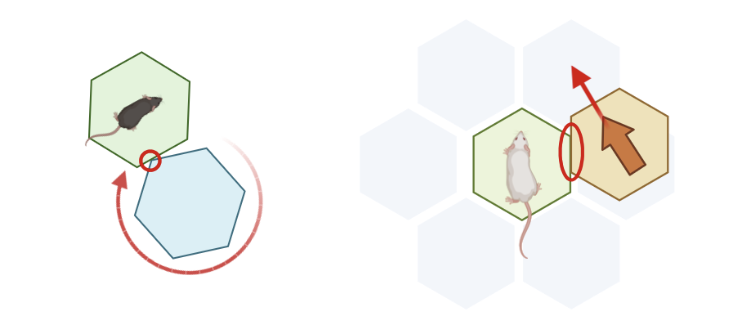
\includegraphics[scale= 0.8]{images/collisions.png}
    \caption{The \textbf{LHS} figure shows how two consecutive hexagonal robot are unable to rotate next to each other. The rotating robot (blue) will collide with the stationary one (green). The \textbf{RHS} shows that direct movement (of the orange robot) to another position in the inner ring is impossible as the platforms will collide.}

\end{figure}

\newpage
\section{Supplementary Material: Functions}

\subsection{Basic moves around the coordinate system}
\label{function:move_around_hex_grid}
\begin{algorithm}
\caption{Function for moving around the hexagonal coordinate space}
 \begin{algorithmic}
 \REQUIRE 'axis' \AND 'step'
   \IF{'axis' is 'x'}
        \STATE$y \leftarrow y + step$
        \STATE$z \leftarrow z - step$
        \RETURN $[x, y, z]$
  \ELSIF{'axis' is 'y'}
        \STATE$y \leftarrow x + step$
        \STATE$z \leftarrow z - step$
        \RETURN $[x, y, z]$
  \ELSIF{'axis' is 'z'}
        \STATE$y \leftarrow x + step$
        \STATE$z \leftarrow y - step$
        \RETURN $[x, y, z]$
   \ENDIF
   
\end{algorithmic}
\end{algorithm}

\subsection{Move to Inner Ring}
\label{function:move to inner ring}
\begin{algorithm}
\caption{Implementation of moving the robot to the inner ring}
 \begin{algorithmic}

\REQUIRE Relative Position between \textit{Animal Robot} \AND \textit{Moving Robot}. This will be a number between 0-5, depending on its position around the animal 
\REQUIRE \textit{Inner Ring Steps} List: [-1, -1, -1, 1, 1, 1]
\REQUIRE \textit{Ring Dimension} List: ['x', 'y', 'z', 'x', 'y', 'z']

\STATE rel pos $\leftarrow$ relative position(\textit{$moving\_robot$})


\end{algorithmic}
\end{algorithm}

\subsection{Get Inner ring coordinates}
\label{function:def_inner_ring}
\begin{algorithm}[H]
\caption{Returns the list of coordinates that are consecutive to the position vector}
\begin{algorithmic}

\REQUIRE Position Vector

inner ring list = [[1, 0, -1], [1, -1, 0], [0, -1, 1],[-1, 0, +1], [-1, 1, 0], [0, 1, -1]]
\FOR{each coordinate in inner ring list}
\STATE new coordinate $\leftarrow$ coordinate + position vector
\STATE append new coordinate to new inner ring list

\ENDFOR
\RETURN new inner ring list


\end{algorithmic}
\end{algorithm}


\subsection{Get Outer ring coordinates}
\label{function:def_outer_ring}
\begin{algorithm}[H]
\caption{Returns the list of coordinates that are two moves away from the position vector}
\begin{algorithmic}

\REQUIRE Position Vector

outer ring = [[2, 0, -2], [2, -1, -1], [2, -2, 0], [1, -2, 1], [0, -2, 2], [-1, -1, 2], [-2, 0, 2], [-2, 1, 1], [-2, 2, 0], [-1, 2, -1], [0, 2, -2], [1, 1, -2]] 
\FOR{each coordinate in inner ring list}
\STATE new coordinate $\leftarrow$ coordinate + position vector
\STATE append new coordinate to new outer ring list

\ENDFOR
\RETURN new outer ring list


\end{algorithmic}
\end{algorithm}





\subsection{Finding relative position}
\label{function:def_relative_position}
\begin{algorithm}[H]
\caption{Function defining the \textit{relative position of a given robot}}
 \begin{algorithmic}
 \REQUIRE \textit{Initial Robot Position Vector, Final Robot Position Vector}
 
 $x, y, z$ is difference in position vectors between \textit{Initial Robot Position Vector} \AND \textit{Final Robot Position Vector}
\IF{$x = 0$ \AND $y = 0$ \AND $z = 0$}
    \RETURN \PRINT{Error Message: Relative Position in not defined here}
\ELSIF{$x = 0$ \AND $x > 0$}
    \RETURN $0$
\ELSIF{$y = 0$ \AND $x > 0$}
    \RETURN $1$
\ELSIF{$z = 0$ \AND $y < 0$}
    \RETURN $2$
\ELSIF{$x = 0$ \AND $x < 0$}
    \RETURN $3$   
\ELSIF{$y = 0$ \AND $x < 0$}
    \RETURN $4$  
\ELSIF{$z = 0$ \AND $y > 0$}
    \RETURN $5$  
\ENDIF

 \end{algorithmic}
\end{algorithm}

\subsection{Change the state of the robots}
\label{function:change_AR_state}
\begin{algorithm}[H]
\caption{Shows the reallocation of the animal robot states after a move has been made by the animal robot}
\function{Reassign robot class}\Comment{Where AR = Animal Robot, NAR = Non-Animal Robot, NNAR = Non-Non-Animal Robot \& State = State of the animal robot}
\begin{algorithmic}
\REQUIRE \textit{New Animal Robot} Class, \textit{Current Robot} Class
\STATE    
\FOR{Each \textit{Robot} in the Maze}
\STATEtunr
\IF {\textit{Robot} Class is \textit{AR} Class \AND the \textit{Robot} Class is \textit{AR} Class}
    \STATE \textit{Robot} Class $\leftarrow$ AR
\ELSIF {\textit{Robot} Class is \textit{New Animal} Class \AND the \textit{Robot} Class is \textit{AR} Class}
    \STATE \textit{Robot} Class $\leftarrow$ NAR
\STATE    
\ELSIF {\textit{Robot} Class is \textit{New NAR} Class \AND the \textit{Robot} Class is \textit{New NAR} Class}
    \STATE \textit{Robot} Class $\leftarrow$ AR
\ELSIF {\textit{Robot} Class is \textit{New AR} Class \AND the \textit{Robot} Class is \textit{New AR} Class}
    \STATE \textit{Robot} Class $\leftarrow$ AR
\STATE    
\ELSIF {\textit{Robot} Class is \textit{New NNAR} Class \AND the \textit{Robot} Class is \textit{New AR} Class}
    \STATE \textit{Robot} Class $\leftarrow$ AR
\ELSIF {\textit{Robot} Class is \textit{New NNAR} Class \AND the \textit{Robot} Class is \textit{New AR} Class}
    \STATE \textit{Robot} Class $\leftarrow$ NNAR
    
    
\ENDIF
\ENDFOR

\end{algorithmic}



\end{algorithm}

\subsection{\textit{Khepera IV} command interpretations}
\label{function:command_interpretation}
\begin{algorithm}
\caption{How the \textit{Khepera IV} interprets command string given to it}
\begin{algorithmic}


% \function{\textit{Khepera IV} command interpretations}\Comment{Input List is a string of numbers}
\REQUIRE Input Command String

\FOR{Each command in \textit{Input Command String}}
    \IF{index of command is even}
        \COMMENT{Interprets the number of turns the robot makes}
        \STATE Rotates the robot 
    \ELSIF{index of command is odd}
        \COMMENT{Interprets the number of moves forwards the robot makes}
        \STATE Moves $command$ number of steps forward
\ENDIF
\ENDFOR{}


\end{algorithmic}
\end{algorithm}




\subsection{Making Command List}

This function makes commands in the format 'number of turns', 'number of steps', 'number of turns', 'number of steps'...

\label{function:make_command_list}
\begin{algorithm}
\caption{From the path list, making a list of commands interpret-able the \textit{Khepera IV} Robot}
\begin{algorithmic}
\REQUIRE Path List of Coordinates which are consecutive to each-other

\FOR{Each Coordinate in Path List}
    %\Comment{To Handle Turns}
    \STATE Get the position vector between the current position of the robot and the next coordinate
    \STATE Get the Relative position of this position vector
    \IF{Direction of Robot is direction of relative position}
        \STATE Append $0$ to command list
        \COMMENT{No Turns Required}
    \ELSIF {Direction is not relative position}
        \STATE $Turns \leftarrow the different in relative position$
        \COMMENT{Get the number of turns between the desired relative position}
        \STATE Append $Turns$ to Command List 
    
    
    \ELSIF {Position of robot is position in command list}
        \STATE Do nothing
    \ELSIF {Position of robot is not position in command list}
        \STATE Append $1$ to command list
        \COMMENT{Step the robot forward 1 step}
    
    
\ENDIF
\ENDFOR

\RETURN Command List


\end{algorithmic}
\end{algorithm}


\subsection{Making Temporary Movement Network}
\label{function:}
\begin{algorithm}
\caption{}
\begin{algorithmic}

\REQUIRE Movement Network
\REQUIRE Moving Robot

\STATE Temporary Movement Network $\leftarrow$ Movement Network Copy 

\FOR{\textit{Robot} in Maze (excluding Moving Robot)}
    \STATE get the consecutive position of the \textit{robot}
    \STATE Add these positions to list
    
 \FOR{Each position in the list}
       \STATE Remove the position from the Temporary Movement Network
\ENDFOR
\ENDFOR


\RETURN Temporary Movement Network

\end{algorithmic}
\end{algorithm}


\subsection{Instantiating of Environment}
\label{function:instantiation}
\begin{algorithm}[H]
\caption{The instantiating of the environment}

\textbf{Instantiate Maze}

\begin{algorithmic}[1]
% \textbf{Instantiate Environment}

\bindent{}
\STATE maze = HexagonMaze($rows$, $columns$, $*name$)
\eindent{}
\\ \textbf{Instantiate Robots}
\bindent{}
\STATE robot1 = PlatformRobot($x$, $y$, $z$, $direction$, $ip\_address$, $concect$, $*name$)
\STATE robot2 = PlatformRobot($x$, $y$, $z$, $direction$, $ip\_address$, $concect$, $*name$)
\STATE robot3 = PlatformRobot($x$, $y$, $z$, $direction$, $ip\_address$, $concect$, $*name$)
\eindent{}

\\ \textbf{Instantiate Animal}
\bindent{}
\STATE animal = Animal($name\_of\_maze$, $*name$)
\eindent{}
\\ \textbf{Point Objects at each-other}
\\ \textit{Robots}
\bindent{}
\STATE robot1.set\_maze($name\_of\_maze$)
\STATE robot2.set\_maze($name\_of\_maze$)
\STATE robot3.set\_maze($name\_of\_maze$)
\eindent{}
\\ \textit{Animals}
\bindent{}
\STATE animal.set\_maze($name\_of\_maze$)
\eindent{}

\\ \textbf{Set the animal robot}
\bindent{}
\STATE robot1.set\_animal\_robot($True$) \algorithmiccomment{robot1 is set to AR}
\eindent{}

\end{algorithmic}
\end{algorithm}

% \subsection{Maze Loop}
% \label{function:maze_loop}
% \begin{algorithm}[H]
% \caption{The sequence of steps that are required for the whole procedure}

% \begin{algorithmic}[1]
% \STATE \textbf{Let the animal make the choice. Then let the maze change the States of the robots} 
% \bindent{}
%     \STATE Animal makes choice
% 	\STATE Change the class of all the robots based on this choice
% 	\STATE Set the position of the animal on top of animal choice
% \eindent{}
% \\ \textbf{Find the pathfinding targets before movement occurs}
% \bindent{}
% 	\STATE Get the NNAR class
% 	\STATE Get the NAR class
% 	\STATE Set the pathfinding targets of NNAR
% 	\STATE Set the pathfinding target of NAR
% \eindent{}
% \\ \textbf{Execute pathfinding for robots}
% \bindent{}
% 	\STATE NNAR step back fron NAR
% 	\STATE and pathfinding to pathfinding target
% 	\STATE NAR step back from AR
% 	\STATE and pathfindin got pathfinding target
% \eindent{}
% \\ \textbf{Move robots into the inner ring}
% \bindent{}
% 	\STATE 13. NAR and NNAR step into inner ring
% \eindent{}


% \end{algorithmic}
% \end{algorithm}

% Note: The maze loop is repeated until the animal reaches the goal



